\section{Microcontroller}

Denne sektion kommer omkring det forskellige moduler, som vores mikroprocesser håndtere. Udover dette konmmer vi også igennem hvilket styresystem vi har valgt og hvorfor.

\subsection{OS}
Det er vigtigt i enhver kode situation, der inkluderer flere tasks, at kunne skifte mellem dem på en fornuftig måde; Dette gøres med en scheduler. Når der skal implementeres en scheduler skal det overvejes hvorvidt det er nødvendigt at lave en designet specielt til projektet, eller om der en en eksisterende der er i stand til at udfører opgaven tilstrækkeligt. I dette project har vi to muligheder til rådighed: FreeRTOS\cite{FreeRTOSorg} eller RTCS.



\subsubsection{FreeRTOS}

FreeRTOS \cite{FreeRTOSorg} er et realtid operativsystem (RTOS), som er en standard løsning som bliver brugt i en mikroprocesser. FreeRTOS giver os muligheden for at bruge preemptiv skedulering, Det vil sige at CPU'en kan sprænge i mellem task og hoppe ud af en task efter behov. Dette bliver styret ud af hvilken prioritet taskén har eller om der en anden task, der for et interrupt den skal holde øje med.
\\
Udover dette har freeRTOS også mange andre funktioner dette projekt kan udnytte. Der er mulighed for at oprette køer, som vil blive nævnt som queues. Disse queues kan man sende events og data til ved hjælp af en funktion der hedder xQueueSend. Hvor der så samtidig med at der en der kan tage noget fra denne queue. 
\\
For at kunne gøre det muligt at flere task's skal kunne til gå disse queue's, dette kan gøres ved at bruge noget det hedder en semafor, som gør at kun en task der har adgang til queue'en indtil semaforen bliver frigjort igen. For at ungå at at styre systemet ikke bliver fastlåst i denne semafor for evigt sætte man en tid, den kan være inde i semaforen.
\\
For at nogle af disse ting kan bliver aktiveret skal der føre oprettes en xQueueHandle og xSemaphoreHandle. Hvorefter de bliver kreeret hved hjælp af xQueueCreate og xSemaphoreCreateMutex. For at bruge xQueueCreate skal der også bruges størrelse af queue'en og hvilken parameter den skal indeholde.
\\
FreeRTOS tilbyder også et shared state memory(SSM), Dette gør det muligt at CPU'en kan hoppe i mellem de forskellige task. F.eks. at det kommer et nød event på UART, som kunne være "STOP\textunderscore EVENT". Dette event gør at den med det samme går over til den case hvor eventet er, og gør som der står, som i dette tilfælde er at bremse motoren.

\subsubsection{RTCS}

Run To Complete Scheduler (RTCS) er en måde at køre ens styresystem på. Den køre som en non preemtiv skedulering, det vil sige at lige så snart CPU'en har forbindelse til en proces/task, så kan den ikke hoppe ud af denne proces/task. I dette system kan der oprettes queue's.
\\
Den har mulighed for at oprette semafoere, som gør at det er kun en queue som kan have adgang til queue'en. For at tilføje data til en queue skal funktion put\textunderscore queue. wait\textunderscore sem bruges til at tilføje en semafor til den specifikke queue.

\subsubsection{Delkonklusion}

Efter vi har set på disse to valg muligheder kan vi se at RTCS vil være næmmere at få til at virker, men at det heller ikke er lige så sikkert, som freeRTOS. Den største begrundelse for at vi vælger at arbjede med freeRTOS over RTCS er at den køre preemtiv. Dette gøre det muligt vis der kommer et vigtigt interrupt at den kan tage CPU'en fra den proces den er i gang med og flytte den over det den mere vigtige proces.

\subsection{Tasks}

\subsubsection{UI}

Den centrale task i systemet er det menu styrede UI system. Denne har primært til opgave at give brugeren mulighed for manuelt at justere, starte eller stoppe systemet, samt at vise vigtige oplysninger såsom nuværende position. Denne styres med drehimpulsgeber og numpad'et, som begge lægger events ind i dens input kø.

\begin{figure}[H]
			\begin{center}
			\includegraphics[scale=0.4]{Billeder/Taskdiagram.PNG}
			\end{center}
			\caption{Task diagram over mikroprocesseren}
			\label{fig:Taskdiagram}
\end{figure}

I figur \ref{fig:Taskdiagram} kan vi se vores task diagram over modulerne i mikroprocesseren.

\subsubsection{Uart}

Uart står for universal asynchronous receiver/transmitter. Dette laver kommunikation mellem to enheder. Så være enhed skal være i stand til at bruge funktion UART. UART transmittere data i form af bytes og deler dem op i bits og sender dem. Modtager skal så kunne samle dem sammen igen til bytes for at læse det.
Vores Uart pinde sider på PORT A, derved skal sysctl aktiveres på port a før den viker. Uart har en init. funktion som bliver kaldt en gang hvor alle register bliver sat up som, f.eks. send og modtag. Der bliver også sat en baut rate, som skal være den samme for sender og modtager.
\\
For at sende data kalder vi funktion uart0\textunderscore putc som tager en karakter. Dette kan både være tal og bogstaver. Der en funktion der hedder uart0\textunderscore rx\textunderscore rdy som venter på at den modstager noget.
\\
For at gøre det nemmer har vi lavet en lille protokol, som skal overholdes før der sendes noget over UART. I figur \ref{fig:UARTCMD} kan ses en liste over de forskellige commands. Et eks. på en UART kald kunne være \texttt{\char`\\}st1803 , som vil sætte tilt delen i 180,3 grader.

\begin{figure}[ht]
			\begin{center}
			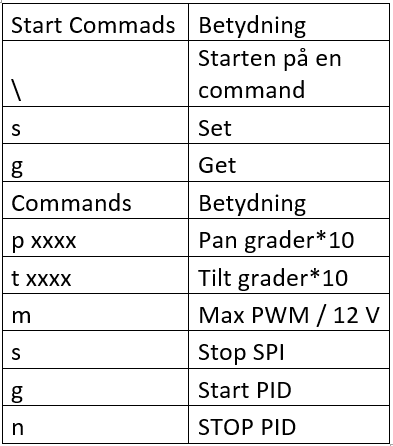
\includegraphics[scale=0.5]{Billeder/UARTCMD.png}
			\end{center}
			\caption{UART commands}
			\label{fig:UARTCMD}
\end{figure}

\subsubsection{LCD}

Den fysiske opsætning af LCD'et kan ses på figur \ref{fig:LCD}, og viser blandt andet at fire databen og R/W benet er forbundet til stel. Med denne opsætning kan man kun skrive til displayet ligesom man er tvunget til at bruge LCD'et i 4-bit mode. Hvis man havde mulighed for at læse fra displayet, kunne man holde øje med et busyflag, der fortæller om LCD'et er optaget, og på den måde sørge for at udnytte displayets tid bedst muligt. Når man kun kan skrive til displayet, er man tvunget til at vente en bestemt tid for at sikre sig at det er klar til at modtage ny data. Til de fleste formål er det dog ikke et problem, at man venter lidt længere end nødvendigt imellem kommandoer. I 4-bit mode kan der kun sendes en nibble ad gangen. For at sende data til displayet, skal dataen skrives ud på de fire databen, derefter flasher man E-benet så LCD'et kan latche og starte behandlingen. RS-benet styrer om den data, der sendes, skal tolkes som data eller en kommando. 

\begin{figure}[ht]
			\begin{center}
			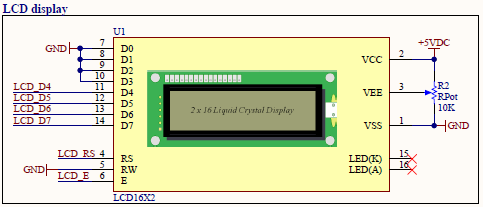
\includegraphics[scale=0.9]{Billeder/LCD.PNG}
			\end{center}
			\caption{LCD pinout}
			\label{fig:LCD}
\end{figure}

Selve LCD-tasken arbejder sammen med resten af systemet ved at afkode et særligt image-format (se figur \ref{fig:LCD_array}), så det vises korrekt på skærmen. Dette image bliver sendt fra display-tasken og indeholder oplysninger om, hvilke karakterer, hvis nogen, der skal skrives til alle 32 synlige adresser på displayet. Udover de 32 karakterer, er der også fire kontrolfelter, som fortæller tasken, hvor cursoren skal placeres efter karaktererne er skrevet ud; om cursoren skal blinke eller bare highlighte nuværende adresse med en streg under karakteren. Det sidste felt bliver sat til at vise adressen, hvor næste karakter skal skrives, når alle 32 karakterer er blevet skrevet første gang. På den måde kan LCD-tasken afgøre om den skal skrive et helt image fra starten, eller bare tilføje en ny karakter til et image der allerede er vist på displayet. Med dette setup kan LCD-tasken finde ud af hvilken ny karakter, der skal tilføjes ud fra den første kontrol-bit, og også hvor cursoren skal placeres efter den er skrevet - hvis den næste adresse, der skal skrives på, er mere end en plads væk, skal cursoren flyttes aktivt. Manipuleringen af images og kontrol-bits foregår i display-tasken - LCD-tasken afkoder bare images, når de bliver tilføjet til dens input-kø.


\begin{figure}[ht]
			\begin{center}
			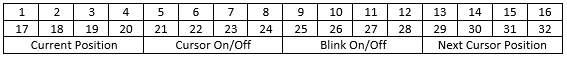
\includegraphics[scale=0.9]{Billeder/LCD_Array.PNG}
			\end{center}
			\caption{LCD Image-format er et array af 36 8-bits størrelser. De første 32 pladser i arrayet repræsenterer de synlige adresser på displayet - de sidste 4 er kontrol-bits.}
			\label{fig:LCD_array}
\end{figure}

\subsubsection{Keypad}

Det udleverede Kit er der tilhørende keypad med 12 knapper fra 0 til 9 og *,\#. Dette keypad virker som knapper, Da er derfor nødvendigt at definere hvad de forskellige knapper skal gøre. For at gøre det simpelt bliver hver knap det som der står på keypad'et. figur \ref{fig:Keypadpins} viser hvordan dens pins at tilsluttet.
\begin{figure}[ht]
	\begin{center}
		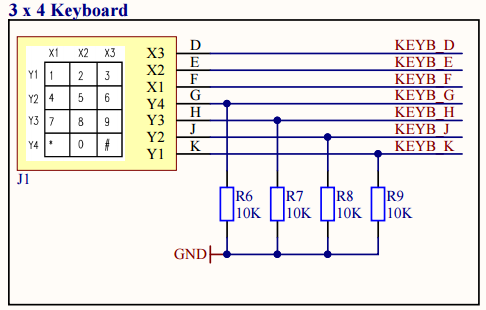
\includegraphics[scale=0.7]{Billeder/Keypadpins.PNG}
	\end{center}
\caption{Keypad pins}
\label{fig:Keypadpins}
\end{figure}
Den har to porte til knyttet som er PORT A og PORT E. Det betyder at vi kan læse på PORT E hvis GPIO pinden på PORT A er aktiv.
\begin{figure}[ht]
	\begin{center}
		\includegraphics[scale=0.7]{Billeder/Keypad.PNG}
	\end{center}
\caption{Keypad struktur}
\label{fig:Keypad}
\end{figure}


På figur \ref{fig:Keypad} kan vi se at vi har givet de forskellige knapper unikke værdier. Dette gøres fordi vi har et array som indeholder alle værdier på keypad’et, som vi så sender ind i bufferen og læse på. For at finde en karakter kigger vi først på alle X værdier (PORT A) igennem og ser om en Y værdi (PORT E) er aktiv og ud fra hvilken X og Y værdi kan vi finde hvilket plads i arrayet ud fra figur \ref{fig:Keypad}
\\
Dette keypad kan blive brugt til at sende data eller manuelt indsætte nogle værdier i mens programmet kører.



\subsubsection{DrehImpulsGeber}

Ved at skrue på drehimpulsgeber kan man inkrementere eller dekrementere en variabel eller sende et event.
Drehimpulsgeberen er en roterende knap som også kan trykkes ned.\\
Drehimpulsgeberen kan sende 30 pulser per rotation.

\begin{figure}[ht]
			\begin{center}
			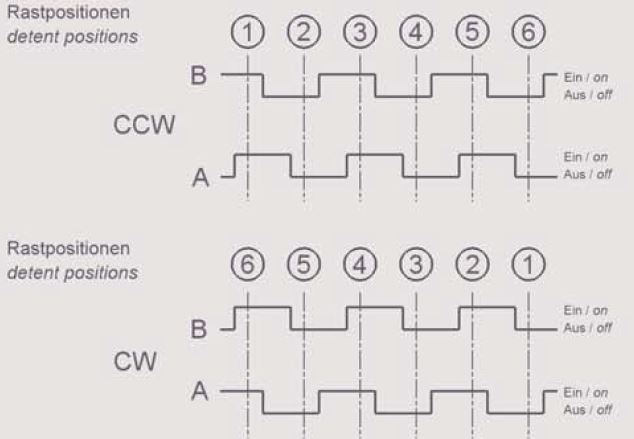
\includegraphics[scale=0.40]{Billeder/DrehImpulsGeber_events.jpg}
			\end{center}
			\label{fig:Impulsgeber_events}
			\caption{Drehimpulsgeber states}
		\end{figure}

for at finde ud af hvilken retning der bliver skruet på impulsgeberen, kigges der på de tidligere states af switchen.
eksempelvist hvis der kigges på figur \ref{Impulsgeber_events} ses det at hvis ben B er højt, og A samtiddig er høj, OG B så falder først og A stadig er høj, så er rotationen en rotation mod uret.


\subsection{Serial Peripheral Interface}
\label{subsec:SPI}

Microcontrolleren der blev udleveret dette semester (TM4C123GH6PM) indeholder 4 SSI (Synchronous Serial Interface) da disse 4 interfaces alle er ens, på undtagelse deres pins, er SSI0 blevet valgt som interface, dvs. port A pin 2 er til SSI0Clk (modulets clock), pin 3 er SSI0Fss (frame signalet), pin 4 er SSI0Rx (modtagelse), og pin 5 er SSI0Tx (afsendelse)

Til SSI modulet er der 3 forskellige data formater:

\begin{itemize}
	\item Texas Instruments Synchronous Serial
		\begin{figure}[ht]
			\begin{center}
			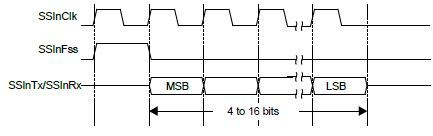
\includegraphics[scale=1]{Billeder/TI_Synchronous_Serial_Frame_Format.jpg}
			\end{center}
			\label{fig:TIFrameFormat}
			\caption{TI Synchronous Serial Frame Format (Single transfer)}
		\end{figure}

	\item Freescale SPI
		\begin{figure}[ht]
			\begin{center}
			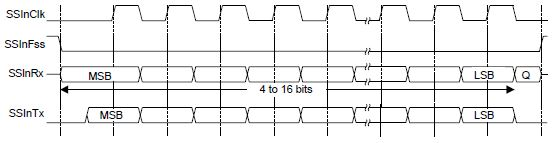
\includegraphics[scale=1]{Billeder/FS_Frame_Format.jpg}
			\end{center}
			\label{fig:FSFrameFormat}
			\caption{FreeScale Frame Format (Single Transfer)}
		\end{figure}
		  
	\item Microwire
		\begin{figure}[ht]
			\begin{center}
			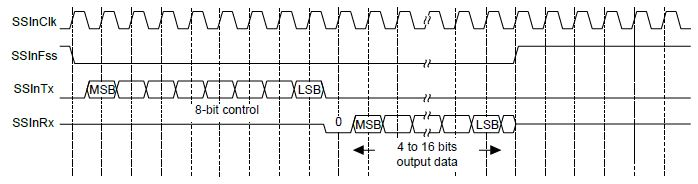
\includegraphics[scale=0.8]{Billeder/MW_Frame_format.jpg}
			\end{center}
			\label{fig:MWFrameFormat}
			\caption{Micro Wire Frame Format (Single Transfer)}
		\end{figure}
\end{itemize}

Da Freescale er den eneste SPI iblandt de tre SSI moduler er det den der blev valgt.

		\begin{figure}[ht]
			\begin{center}
			\includegraphics[scale=0.8]{Billeder/Spi_Setup.jpg}
			\end{center}
			\label{fig:SPI_Setup}
			\caption{Setup af Freescale SPI}
		\end{figure}

For at lave et Freescale setup skal SSI modulet deaktiveres, også kan microcontrolleren sættes som master ved at skrive nul til control registret.
Derefter skal clock configurations registret sættes til 0 så vi bruger system clocken.
Der ønskes en 2 Mbps clock bruges følgende ligning

\begin{align*}
2*10^6 bps &= \dfrac{16*10^6 Hz}{CPSDVSR * (1 + 0)}\\
CPSDVSR &= \dfrac{16*10^6 Hz}{2*10^6 bps}\\
CPSDVSR &= 8
\end{align*}

Så sættes kontrol registret for SSI0 til 0xF da bit 3:0 angiver data størrelse, 0xF er så 16-bit data. Samtidig bliver Freescale SPI sat op, da bit 4 og 5 bestemmer frame formatet, og hvis de begge er lave betyder det at Freescale er valgt. 
og igen sættes bit 1 i kontrol registret for SSI1 til høj så SSI'en er aktiveret.

\subsection{PID-Controller}

PID-controllerens opgave består i at beregne sig frem til et passende PWM-signal, til at regulere motoren med, ud fra forskellen imellem motorens ønskede og faktiske position. Dette PWM-signal skal drive fejlen i 0 på en måde, der opfylder projektets designmål. Beregningen er styret af de tre konstanter $K_{P}$, $K_{I}$ og $K_{D}$, som man, igennem en analyse af systemets opførsel, beregner sig frem til. Denne analyse antager et ideelt system, hvor man hele tiden med uendeligt små tidsintervaller kan justere controllerens output. Det er ikke muligt at implementere en controller i den form, så der vil være en forskel på den programmerede og den modellerede controllers opførsel.


\subsubsection{Basal Virkemåde}

Selve udregningen af outputtet sker ved, at controlleren med jævne mellemrum kigger på setpointet for en motor, og sammenligner det med motorens faktiske position. Dette giver en fejlværdi som der løbende holdes øje med. 
\begin{itemize}
\item For at finde proportionaltermet ganges konstanten $K_{P}$ på fejlværdien
\item For at finde integraltermet ganges konstanten $K_{I}$ på en løbende summering af arealet under fejlen. Dette areal findes ved at gange $dt$ på fejlen, og så lægge det til hver gang udregningen køres igennem. På figur \ref{fig:Riemann} kan man se, hvordan integralet hele tiden vokser, så længe en fejl er til stede.
\item For at finde differentialtermet ganges konstanten $K_{D}$ på forskellen imellem den nuværende fejl og den forrige fejl delt med dt. Det svarer til at beregne $\Delta e/\Delta t$.
\end{itemize}

\begin{figure}[ht]
	\begin{center}
	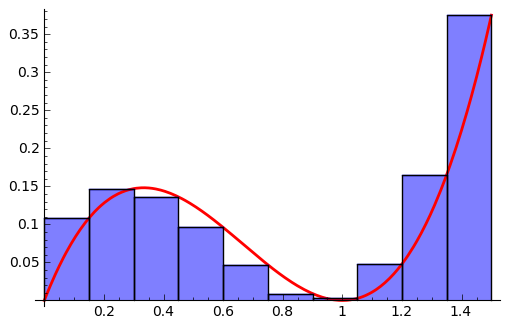
\includegraphics[scale=0.8]{Billeder/RiemannSum.png}
	\end{center}		
	\caption{Her ses en visualisering af det løbende integral der udregnes i starten af hver sample-periode. Arealet dækket af alle de blå bjælker viser størrelsen af integralet, og den røde kurve viser hvordan fejlen ændrer sig over tid.}
	\label{fig:Riemann}
\end{figure}

Når de tre termer er fundet, summeres de for at finde det endelige output fra udregningen. Dette output er i sig selv ikke brugbart til at finde en duty cycle som motoren skal reguleres med. Man er nødt til at definere et interval som outputtet kan operere indenfor. På den måde kan man, ved at finde ud af hvor outputtet befinder sig i intervallet, mappe denne position til en duty cycle mellem 0 og 255. På figur \ref{fig:Mapping} kan man se en visualisering af denne mapping. Hvis outputtet er negativt betyder det at retningen skal ændres på motoren, men det ændrer ikke noget på hvilken duty cycle, der skal sendes i sidste ende.

\begin{wrapfigure}{R}{0.5\textwidth}
\vspace{-20pt}
	\begin{center}
	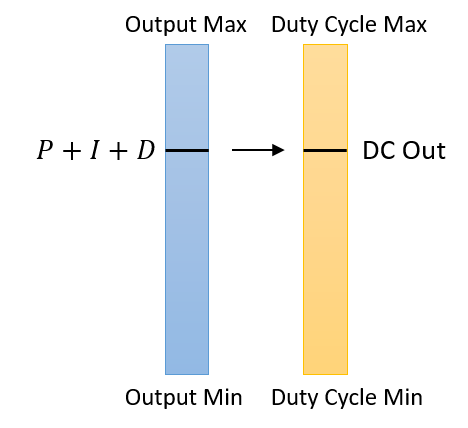
\includegraphics[width=0.5\textwidth]{Billeder/Mapping.png}
	\end{center}		
	\vspace{-10pt}
	\caption{Her ses hvordan PID-outputtet mappes til en tilsvarende duty cycle}
	\label{fig:Mapping}	
\vspace{-20pt}
\end{wrapfigure}
\paragraph{Duty Cycle}

Det har en ret stor betydning hvilke duty cycles man kan sætte som output. Med duty cycles under 15 $\%$ kan man, for eksempel næsten ikke slæbe systemet rundt, og når man over 75 $\%$ kan systemet justere så voldsomt at selve platformen, rammerne er monteret på, begynder at flytte sig rundt på bordet. Af den grund blev der sat et interval mellem 15 $\%$ og 60 $\%$ som controlleren kunne justere indenfor. For at forhindre systemet i at oscillere omkring set point'et med en duty cycle på 15 $\%$ låses motoren, når fejlen er 0.

\paragraph{Skalering}

Et problem ved at bruge FreeRTOS som platform er, at det ikke er muligt at regne med floating point tal. Microcontrolleren kan fint arbejde med dem, da den har et floating point unit, men port mappet til FreeRTOS er lavet til en processor der ikke har en. Det giver problemer når FreeRTOS laver kontekst skift. Den kan ikke finde ud af at gemme floats i memory, når der skiftes imellem tasks. Så hvis der benyttes floats, så trapper styresystemet til et fault interrupt.

Af den grund er alle udregninger nødt til at foregå på heltal. For at kunne slippe afsted med det, er man nødt til at skalere operanderne i udregningerne, da der tit er tale om kommatal i en eller anden størrelsesorden. Den elegante og mest effektive løsning fås ved at bruge \textit{fixed point} aritmetik. Det kan dog være lidt svært at tyde tallene, når man læser koden, da de bliver konverteret til en størrelse der ikke, ved første øjekast, har nogen relation til det oprindelige tal. En simplere løsning i samme boldgade, som vi også endte med at bruge, er at skalere tallene med størrelsesordner af faktor 10. Det gør tallene ret store, men i kraft af at microcontrolleren arbejder med 32 bits ad gangen, er der ret højt til loftet. Det er også lettere for normale mennesker at arbejde med tal i base 10.

Det er vigtigt at sørge for at alle termerne bliver skaleret lige meget, så forholdet imellem termerne ikke ændres. De to ting der er nødvendige at skalere er $dt$ og gainet til controlleren, da de begge er i størrelsesorden $10^{-3}$. Det er så her man skal holde tungen lige i munden, for P-termet bliver kun påvirket af gainet og både I- og D-termet bliver påvirket af gain og $dt$, men D-termet bliver påvirket af $dt$-skaleringen modsat i forhold til I-termet. Så det vil sige at man, med en skaleringsfaktor på $10^4$, ender med et P-term skaleret med $10^4$, et I-term skaleret med $10^8$ og et D-term skaleret med $10^0$. Det skal der selvfølgelig justeres for, så outputtet giver mening.

\paragraph{Integral Windup}

Et problem med PID-controlleren er integral windup. Integral windup er, når arealet under fejlen vokser sig så stort at I-termet kommer til at dominere outputtet. Det er et stort problem for især langsomme systemer, som bruger lang tid på at drive fejlen i 0. Så længe der er en fejl til stede, vil integralet vokse sig større. Det kan blive så stort at systemet er nødt til at tilbringe lang tid med en modsatrettet fejl for at komme tilbage til set point - det er ikke en opførsel man er interesseret i. I de fleste tilfælde er integralets eneste vigtige bidrag at forhindre steady state fejl ved at "trække" systemet på plads, når man er tæt på målet. Af den grund er der mange implementeringer der simpelthen ignorerer integraltermet, når fejlen er over en vis størrelse. En anden mulighed er at sætte et loft på, hvor stort integralet kan blive. Til dette projekt blev begge metoder benyttet, da det viste sig at være ret problematisk at kontrollere integratoren. 

\subsubsection{PID Task}

PID task'en har to tilstande: idle og running. I idle-tilstanden ventes der på et \texttt{PID\_START\_EVENT}, der skifter tilstanden til running. I running-tilstanden køres funktionen \texttt{PID\_update()} med faste intervaller. Denne funktion sørger for at hente set point og den fysiske position af rammerne for både pan- og tilt-systemet. Det kræver kommunikation med SPI-task'en der fungerer som bindeledet til selve systemet. Kommunikationen er styret fuldstændig af PID-task'en, der bare benytter de services som SPI-task'en tilbyder. Når \texttt{PID\_update()} bliver kaldt, beregnes outputtet for pan-systemet og derefter for tilt-systemet. Når det er sket sendes et \texttt{SET\_PWM\_EVENT} til SPI-task'en som sender informationen videre til FPGA'en. Efter eventet er sendt sover PID-tasken i 5 ms, hvorefter den sender et \texttt{GET\_POS\_EVENT} til SPI-task'en, som henter den nuværende position af både pan- og tilt-systemet fra FPGA'en og gemmer den i shared state memory. Når den er færdig med det sendes et \texttt{PID\_UPDATE\_EVENT} tilbage til PID-task'en som starter cycklusen forfra. Hele processen kan ses på figur \ref{fig:PID_update}.

\begin{wrapfigure}{L}{0.5\textwidth}
\vspace{-20pt}
	\begin{center}
	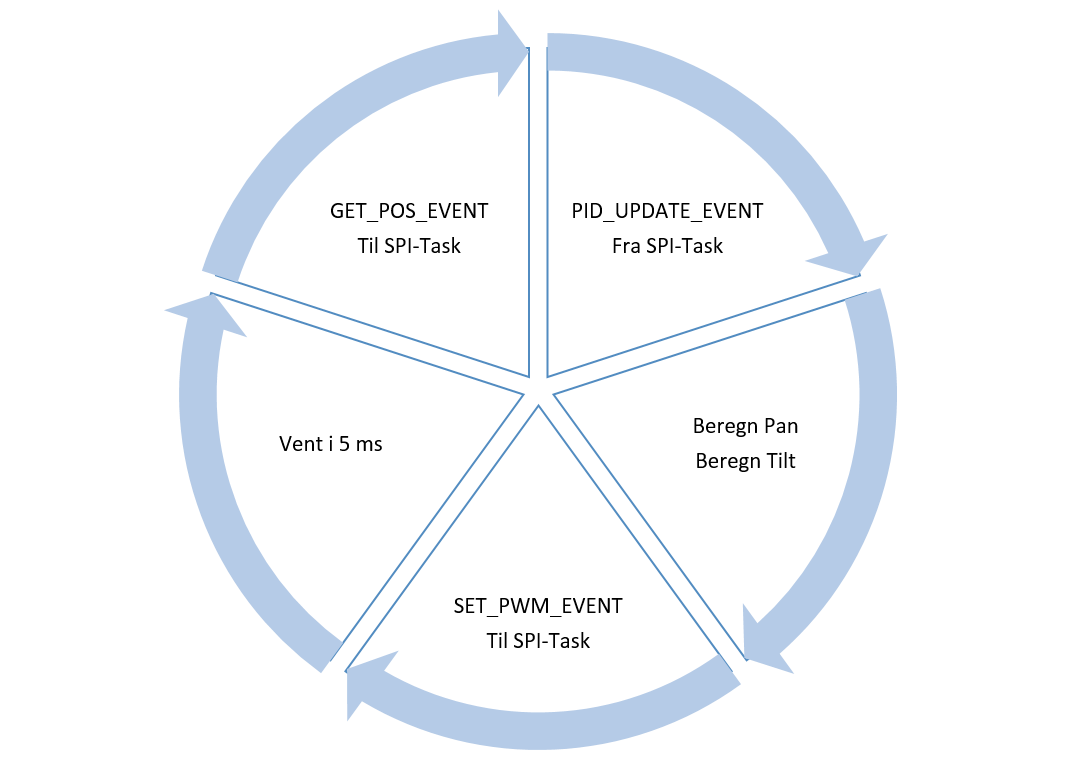
\includegraphics[scale=0.5]{Billeder/PID_update.png}
	\end{center}		
	\vspace{-10pt}
	\caption{Her ses en visualisering af den cyklus som PID-task'en styrer, når den er i running-tilstanden}
	\label{fig:PID_update}
	\vspace{-20pt}
\end{wrapfigure}

\paragraph{Filter}
En alternativ måde at gribe implementeringen an på, er at lave controlleren som et filter. Det kan lade sig gøre ved at mappe overføringsfunktionen over i z-domænet og den vej igennem finde filterkoefficienterne. Denne metodik tillader implementeringen af andre controller-typer som fx lead- og lag-controllere, da lettere man kan implementerer flere slags overføringsfunktioner.

\subsubsection{Delkonklusion}

PID-controllleren blev implementeret med en sample frekvens på 200 Hz. Dette afspejler ikke helt præcist den modellerede controller, men det er tæt nok på til at kunne opfylde kravene til projektet. Der kunne også have været brugt \textit{fixed point} aritmetik til udregningerne på microcontrolleren, men det blev vurderet at det skabte flere problemer end det løste under udviklingen. Det er noget som kunne tages op igen på et senere tidspunkt. For at slippe af med integral windup blev der sat et loft på hvor stort integralet kunne blive, og det blev slet ikke brugt, når fejlen var over en bestemt størrelse. For at forhindre oscillationer omkring set point låses motoren når fejlen er 0. En filterimplementering blev ikke udforsket, men kunne helt klart være en mulig forbedring af systemet i fremtiden.

\subsection{Løse funktionaliteter}

\subsubsection{Koordinat oversættelse}

Da pan og tilt rammen har en præcision på en tredjedel grad, og det samtidigt er et primært krav at denne skal kunne fungerer med input i form af polære koordinater, er det nødvendigt at have en koordinat oversættelse fra de inputtede koordinater. Denne oversættelse skal nødvendigvis tage højde for at de fysiske begrændsninger systemet har. Oversættelsen skal derfor lave en oversættelse i pan delen der afspejler at denne kun kan bevæge sig lidt over 180 grader uden at der opstår problemer med de ledninger der styrer tilt delen. Dette er dog slet ikke nok til at lave et effektivt teleskop system.
\\
Løsningen til dette er at tilt delen bliver spejlet omkring origo når systemet forsøger at pege mod et punkt der ligger i området mellem 90 og 270 grader. Grunden til at systemet kan bevæge sig 90 grader til hver side, omend dette kan virke irrationelt, er at dette er positionen af den hall sensor der benyttes til at nulstille koordinat systemet på FPGA'en. Nulpunktet i tilt delen af teleskop systemet er positioneret direkte opad, da dette både gjorde det mindre kompliceret at spejle det, og samtidig passede bedre overens med det polære koordinat system. Der kunne argumenteres for at det ville være nemmere også at sætte dennes nulpunkt der hvor hall sensoren nulstiller FPGA'en, men dette blev valgt fordi det er mere modulært at gå efter et system der mere matematisk intuitivt.
\\
En stor fordel ved denne koordinat oversættelse er at den eliminerer nødvendigheden for et sikkerhedssystem på microcontrolleren. Dette er naturligt en del af koordinat oversættelsen, da alt mellem 90 og 270 grader på pan systemet, som er de områder hvor der kan ske mekaniske skader, slet ikke er aktuelt, på grund af spejlingen af koordinaterne. Det skal dog noteres at dette ikke eliminerer behovet for et sikkerhedssystem på FPGA'en, som der stadig er brug for i tilfælde af et der forekommer problemer med microcontrolleren, så som en løs forbindelse, en fejl der får hele microprocessoren til at fryse, eller overshoot der går ud over den sikkerheds grændse der er blevet besluttet.




















